\documentclass{article}
\usepackage{tikz}
\usetikzlibrary{arrows}
\begin{document}
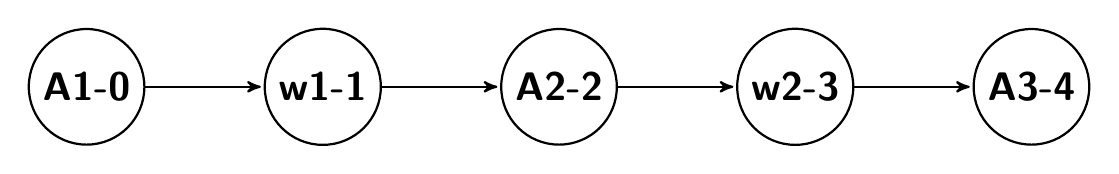
\begin{tikzpicture}[->,>=stealth',shorten >=1pt,auto,node distance=3cm,
                    thick,main node/.style={circle,draw,font=\sffamily\Large\bfseries}]
  \node[main node] (1) {A1-0};
  \node[main node] (2) [right of=1] {w1-1};
  \node[main node] (3) [right of=2] {A2-2};
  \node[main node] (4) [right of=3] {w2-3};
  \node[main node] (5) [right of=4] {A3-4};
  
  \path[every node/.style={font=\sffamily\small}]
    (1) edge [right] node[left] {} (2)
    (2) edge [right] node[left] {} (3)
    (3) edge [right] node[left] {} (4)
    (4) edge [right] node[left] {} (5);
\end{tikzpicture}
\end{document}